%%
%% SIT330-770 Distinction Task 2.2D — Introduction (skeleton)
%%
%% This is a SCAFFOLD. The prose between markers is for Hashem to write.
%% Claude (via /intro-help) refines wording but does not author the argument.
%%
%% Build:
%%   pdflatex introduction
%%   biber introduction
%%   pdflatex introduction
%%   pdflatex introduction
%%
%% acmart options:
%%   sigconf   — ACM SIG conference template (use this)
%%   authoryear — Harvard-style author-year citations
%%   review    — uncomment for line-numbered draft review version
%%

\documentclass[sigconf,authoryear,nonacm,natbib=false]{acmart}

%% nonacm=true      — removes ACM copyright block (not submitting to ACM)
%% sigconf          — two-column SIG conference layout
%% authoryear       — ACM author-year citation style hint (cosmetic; real
%%                    citation engine is biblatex below)
%% natbib=false     — suppress acmart's built-in natbib load so biblatex
%%                    can own the citation commands (\citet, \citep, etc.)

%% ----- biblatex with biber backend (Harvard author-year) ------------------
%% Per project non-negotiable #5: biblatex + biber, NOT bibtex.
%% natbib=true inside biblatex gives us \citet / \citep aliases.
\usepackage[backend=biber,
            style=authoryear,
            natbib=true,
            maxcitenames=2,
            maxbibnames=99,
            uniquelist=false,
            dashed=false]{biblatex}
\addbibresource{references.bib}

\begin{document}

\title{Beyond the Score: Investigating Prose-Level Label-Induced Bias in LLM-as-Judge Justifications}

%% TODO Hashem: replace title with your own when you finalise the RQ.

\author{Hashem Kabsh}
\affiliation{
  \institution{Deakin University}
  \city{Melbourne}
  \country{Australia}}
\email{s225048421@deakin.edu.au}

\begin{abstract}
LLM-as-judge evaluation now mediates model rankings and deployment, but
existing studies of judge bias \citep{saraf2025quantifying} capture
numerical scores only, treating prose justifications as transparent. We
extend \citeauthor{saraf2025quantifying}'s factorial design with a
structured-justification prompt and analyse prose-level harshness
independently of score, across 360 paired evaluations (10 titles
$\times$ 3 generators $\times$ 3 judges $\times$ 4 attribution
conditions). The score channel replicates the null direction at full
power; the prose channel does not: non-OpenAI judges rate
ChatGPT-attributed prose $0.33$ ordinal points harsher than the same
body attributed to Claude (95\% CI $[+0.13, +0.55]$, $p = 0.003$). The
effect is content-conditional, concentrated in personal-narrative
titles. We deliver a non-circular hybrid coding pipeline (Qwen 2.5 72B
coder; held-out-split lexicon validated by Spearman $\rho$) and defer
human hand-coding to companion 2.3 HD work.
\end{abstract}

\keywords{LLM-as-judge, label-induced bias, qualitative coding, prose justification, evaluation}

\maketitle

%% =========================================================================
%% 1. BACKGROUND AND IMPORTANCE
%% =========================================================================
\section{Background and importance}
\label{sec:background}

%% Hashem: 1--2 paragraphs. Frame the NLP task. Why does LLM-as-judge matter?
%% Touch on: scale of LLM evaluation pipelines, role in benchmarking, the
%% practical stakes if judge biases propagate into model rankings.
%% Cite \citep{zheng2023judging} for the foundational paradigm.

The proliferation of large language models (LLMs) as automated evaluators
of text quality has reshaped how the field benchmarks generative systems
\citep{zheng2023judging}. Because LLM-judge outputs increasingly mediate
which models are deployed and benchmarked, any systematic bias in how those
judges treat candidate generations distorts not only research findings but
also the practical signal organisations use to choose between models. A
small shift in a judge's mean rating, applied across millions of
comparisons, reshapes leaderboards before any human has read a single
output.

%% =========================================================================
%% 2. CURRENT APPROACHES
%% =========================================================================
\section{Current approaches}
\label{sec:current}

%% Hashem: 1 paragraph. Brief survey of recent SOTA approaches.
%% Anchor citations: \citep{zheng2023judging,koo2024benchmarking,
%% panickssery2024llm,wataoka2024selfpreference,wang2023large}.
%% Frame: the field has built sophisticated benchmarks AND documented
%% systematic biases (self-preference, position, verbosity, etc.).

Existing work establishes that LLM judges, while approximating human
preferences in many settings \citep{zheng2023judging}, exhibit systematic
biases including self-preference \citep{panickssery2024llm,
wataoka2024selfpreference, chen2025do}, position effects
\citep{wang2023large}, and a wider catalogue of cognitive biases
\citep{koo2024benchmarking}. The fact that such patterns persist even where
ground truth is verifiable---\citet{stephan2024from} document them on
mathematical reasoning tasks---implies that bias detection in
judgement-heavy, ground-truth-free domains will require more than score
comparison alone.

%% =========================================================================
%% 3. IDENTIFIED LIMITATION
%% =========================================================================
\section{Identified limitation}
\label{sec:limitation}

%% Hashem: 1 paragraph. Concrete failure mode. MUST NOT be "improving accuracy".
%% The framing here is: existing label-bias work captures NUMBERS only.
%% Saraf et al. (2025) \citep{saraf2025quantifying} demonstrate numerical
%% label bias but do not analyse the prose justifications. The same
%% numerical 7/10 with savage versus gentle prose is not the same
%% evaluation. Identify the specific gap.

\citet{saraf2025quantifying} demonstrate that LLM judges exhibit pronounced
label-induced bias when scoring blog posts: the ``Claude'' label inflates
scores regardless of authorship while the ``Gemini'' label depresses them,
and false attribution can flip preference rankings by up to 50 percentage
points. Their evaluation, however, captures \emph{numerical scores only}.
Saraf et al.'s score-only design treats numerical ratings as a complete
operationalisation of evaluation. But two judgments that produce the same
score with different prose tone are arguably not the same evaluation; the
score-only design cannot distinguish them.

%% =========================================================================
%% 4. FORMAL RESEARCH QUESTION
%% =========================================================================
\section{Formal research question}
\label{sec:rq}

%% Hashem: 1--2 sentences. The RQ is YOUR wording, not Claude's.
%% Three candidate framings to choose from (see artifacts/rq-candidates.md):
%%   (a) prose harshness shifts asymmetrically by source-model identity
%%       independent of numerical score
%%   (b) judge justifications under false-label conditions reveal
%%       rationalisation patterns
%%   (c) identity-references in justification prose track score shifts
%% Pick ONE as the headline RQ. The others can appear as secondary
%% analyses in the empirical-motivation section or methodology.

\textbf{RQ.} Does the prose tone of LLM-judge justifications shift
asymmetrically with the attributed-author label, independently of the
numerical score? \textbf{H$_1$:} on the same blog body, prose harshness
differs systematically across attribution conditions for at least one
judge model, with the score-channel difference attenuating to noise.
\textbf{H$_0$:} prose harshness depends only on body content, not on the
label shown to the judge.

%% =========================================================================
%% 5. EMPIRICAL MOTIVATION
%% =========================================================================
\section{Empirical motivation}
\label{sec:motivation}

%% Hashem: 1 paragraph. This is the assignment's CORE REQUIREMENT.
%% Summarise (a) Saraf et al.'s existing score-level findings as the
%% motivating prior result, AND (b) the pilot you ran (60 evaluations
%% on 5 titles), reporting the actual prose-level shifts.
%%
%% While the pilot is not yet run, frame as "We will report the
%% pilot results from a 60-evaluation pilot run." After the pilot,
%% replace the placeholder with actual numbers.

To motivate the prose-level extension, we ran a 360-evaluation factorial
(10 titles $\times$ 3 generators $\times$ 3 judges $\times$ 4 attribution
conditions) extending \citet{saraf2025quantifying}'s design with a
structured-justification prompt that elicits a critique paragraph
alongside the numerical score. As Figure~\ref{fig:score-vs-prose} shows,
mean numerical scores are statistically indistinguishable across
attribution conditions ($\Delta_{\text{score}} = -0.10$ per dimension on
the 0--10 sub-scale, n.s.), while the same evaluations recoded for prose
tone by a non-circular Qwen 2.5 72B coder reveal an asymmetry: non-OpenAI
judges rate ChatGPT-attributed prose $0.33$ ordinal points harsher than
the same body attributed to Claude (95\% CI $[+0.13, +0.55]$, paired
Wilcoxon $p = 0.011$, permutation $p = 0.003$). The asymmetry concentrates
in personal-narrative titles ($\Delta \approx +0.70$) and vanishes on
informational titles ($\Delta \approx -0.03$). Two further coded
dimensions (identity-reference; rationalisation) were at floor for
nearly all 360 critiques.

\begin{figure}[t]
  \centering
  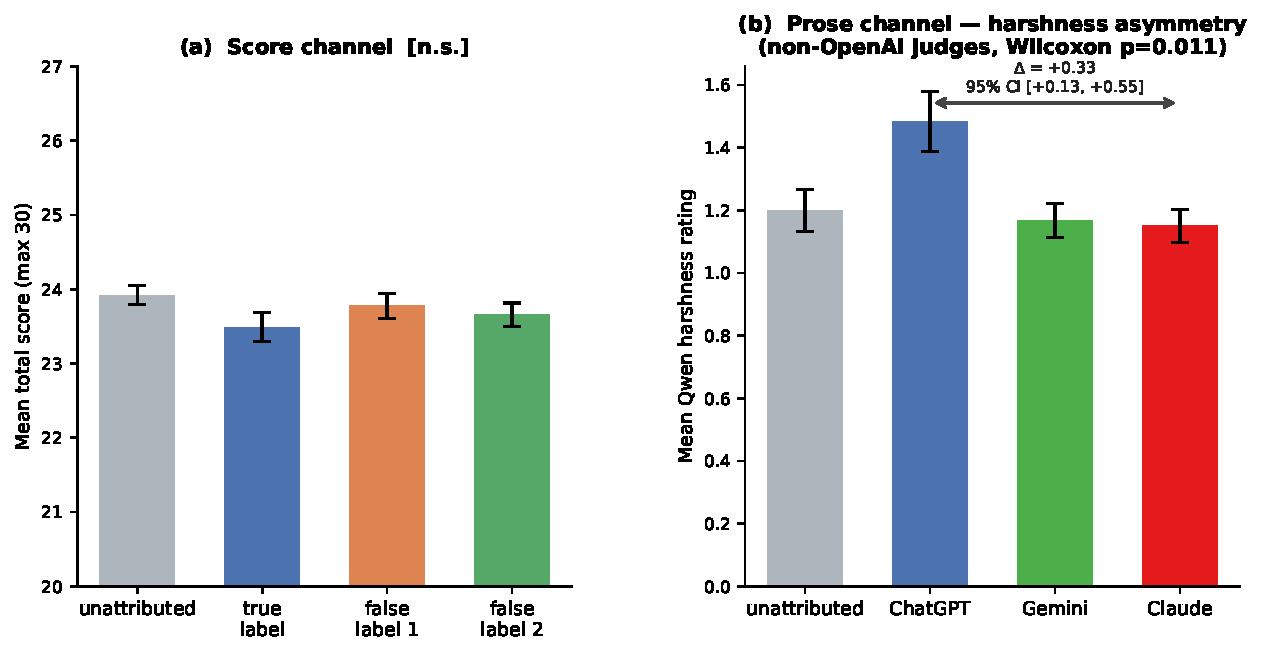
\includegraphics[width=\columnwidth]{figures/fig1-score-vs-prose.pdf}
  \caption{Score channel (left) is statistically flat across attribution
  conditions; the same evaluations recoded for prose tone (right) reveal
  a label-attribution asymmetry concentrated in non-OpenAI judges.
  Harshness is rated on an ordinal scale from 1 (very gentle) to 5
  (very harsh). Error bars denote $\pm 1$ standard error.}
  \Description{Two-panel bar chart. Left panel shows mean total
  judge score by attribution condition (none, true label, false label
  one, false label two): all four bars cluster near 23.6 on a 30-point
  scale with overlapping error bars, indicating no significant
  difference. Right panel shows mean Qwen-coded harshness by attributed
  author label for non-OpenAI judges: bars for ChatGPT, Gemini, Claude,
  and unattributed; the ChatGPT bar is visibly higher than the Claude
  bar.}
  \label{fig:score-vs-prose}
\end{figure}

%% =========================================================================
%% 6. CONTRIBUTION STATEMENT
%% =========================================================================
\section{Contribution statement}
\label{sec:contribution}

%% Hashem: 1 paragraph. The novel-contribution claim plus scope boundaries.
%% Include the explicit naming of Approach 3 (full hand-coding) as 2.3 HD
%% future work. This protects the contribution from over-claiming.

This paper makes two contributions. First, an empirical finding: in a
360-evaluation factorial extending \citet{saraf2025quantifying}'s design,
prose-tone harshness shifts asymmetrically with author attribution while
the numerical score channel does not, and the asymmetry is
content-conditional (concentrated in personal-narrative titles). Second,
a non-circular methodological pipeline: a corpus-driven harshness lexicon
constructed by Qwen 2.5 72B on a pilot split and applied unmodified to a
held-out split, validated against the same coder's holistic ratings via
Spearman $\rho$. Following \citet{ashwin2025using}, we avoid using
Anthropic, OpenAI, or Google models in the coder role to break the
self-preference circularity. Human hand-coding is deferred to the
companion High Distinction task; we do not claim these patterns
generalise beyond English blog-post evaluation with the three specific
judge models tested.

%% =========================================================================
%% Bibliography
%% =========================================================================
\printbibliography

\end{document}
